\def \initvolwidth {0.5}
\def \initvolheight {0.4}
\def \initvolhorshift {0cm}
\def \initvolvertshift {-2cm}

\begin{figure}
  \centering
  \vspace*{\initvolvertshift}
    \hspace*{\initvolhorshift}\subfloat[Vanderpol]{
    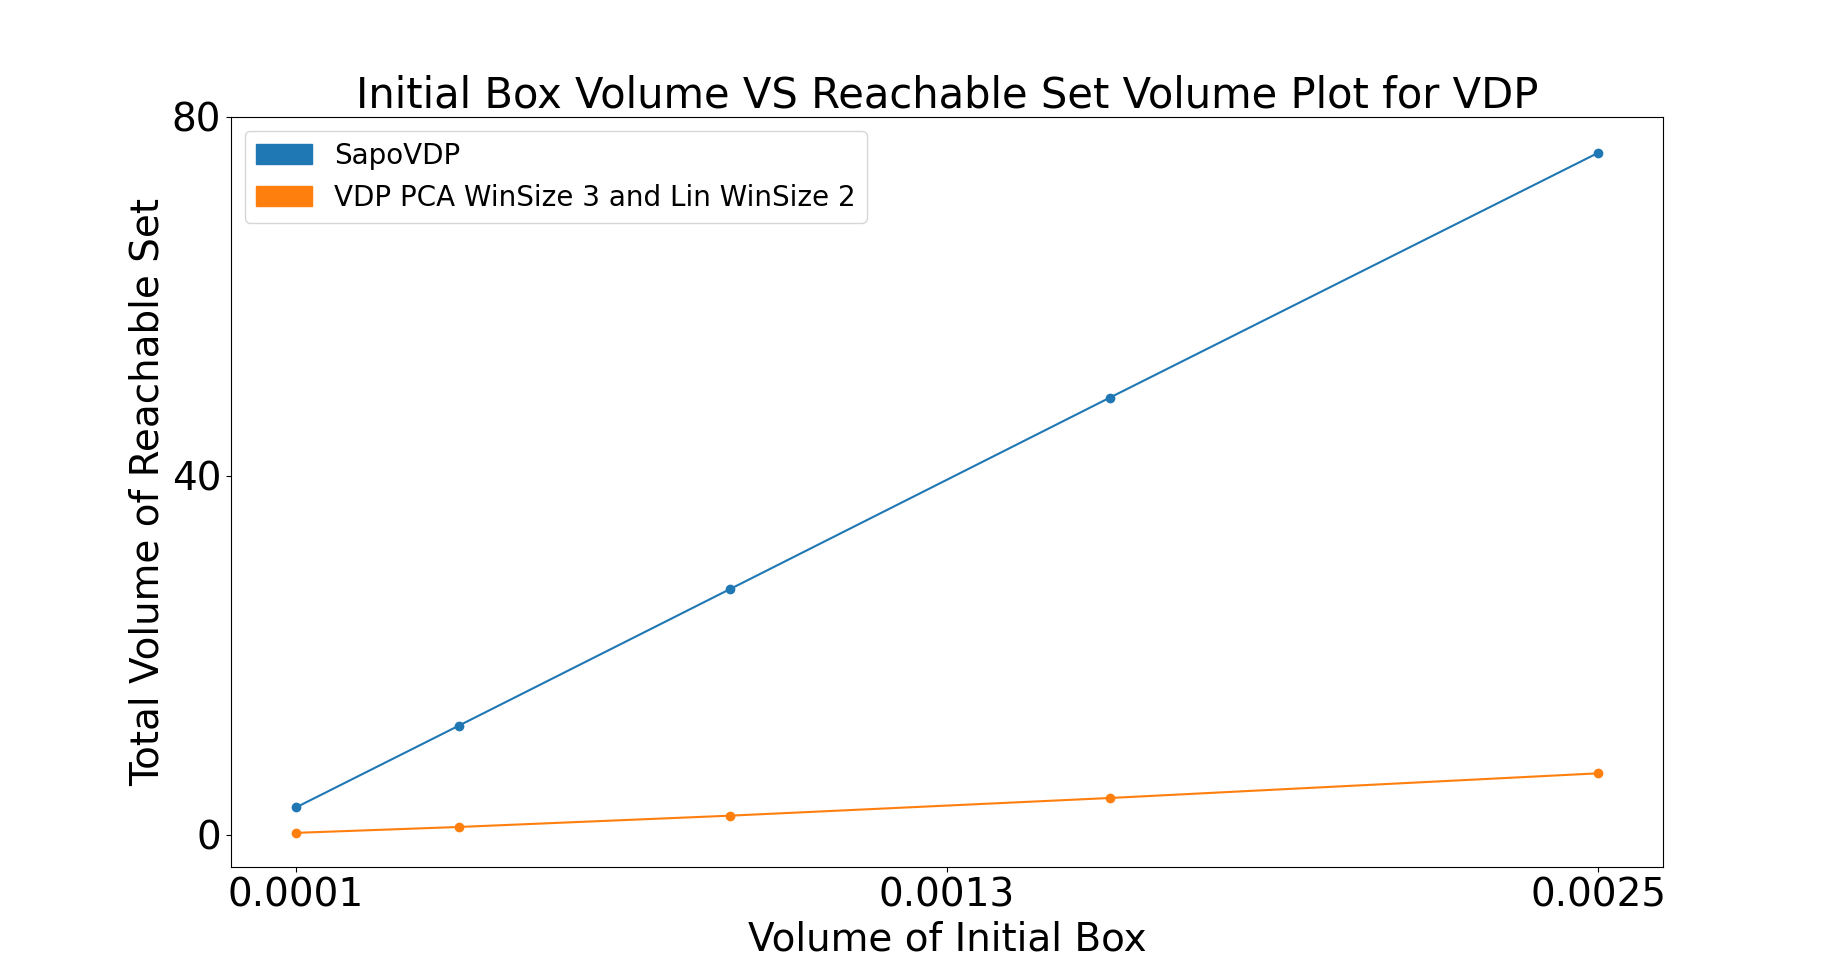
\includegraphics[width=\initvolwidth\textwidth, height=\initvolheight \textwidth]{figures/InitVolVSReachVol/VDPInitReachVol.png}
  }
  \subfloat[Jet Engine]{
  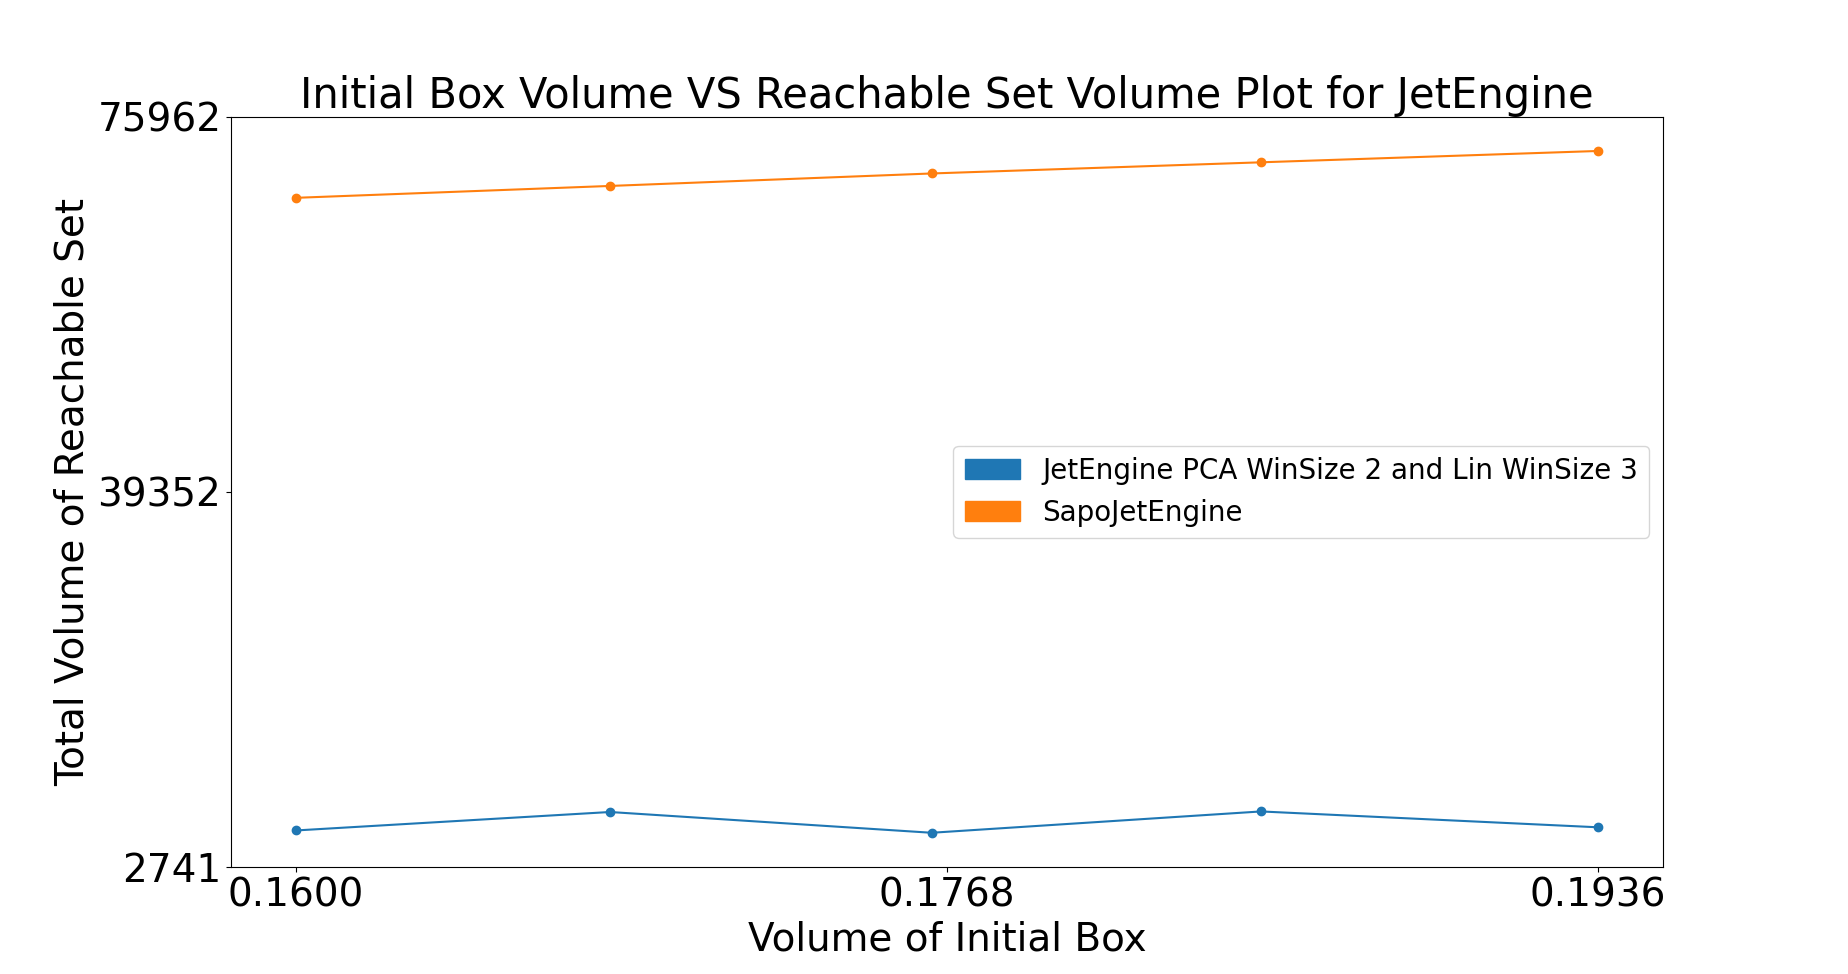
\includegraphics[width=\initvolwidth\textwidth, height=\initvolheight \textwidth]{figures/InitVolVSReachVol/JetEngineInitReachVol.png}
  }

  \hspace*{\initvolhorshift}\subfloat[Neuron]{
    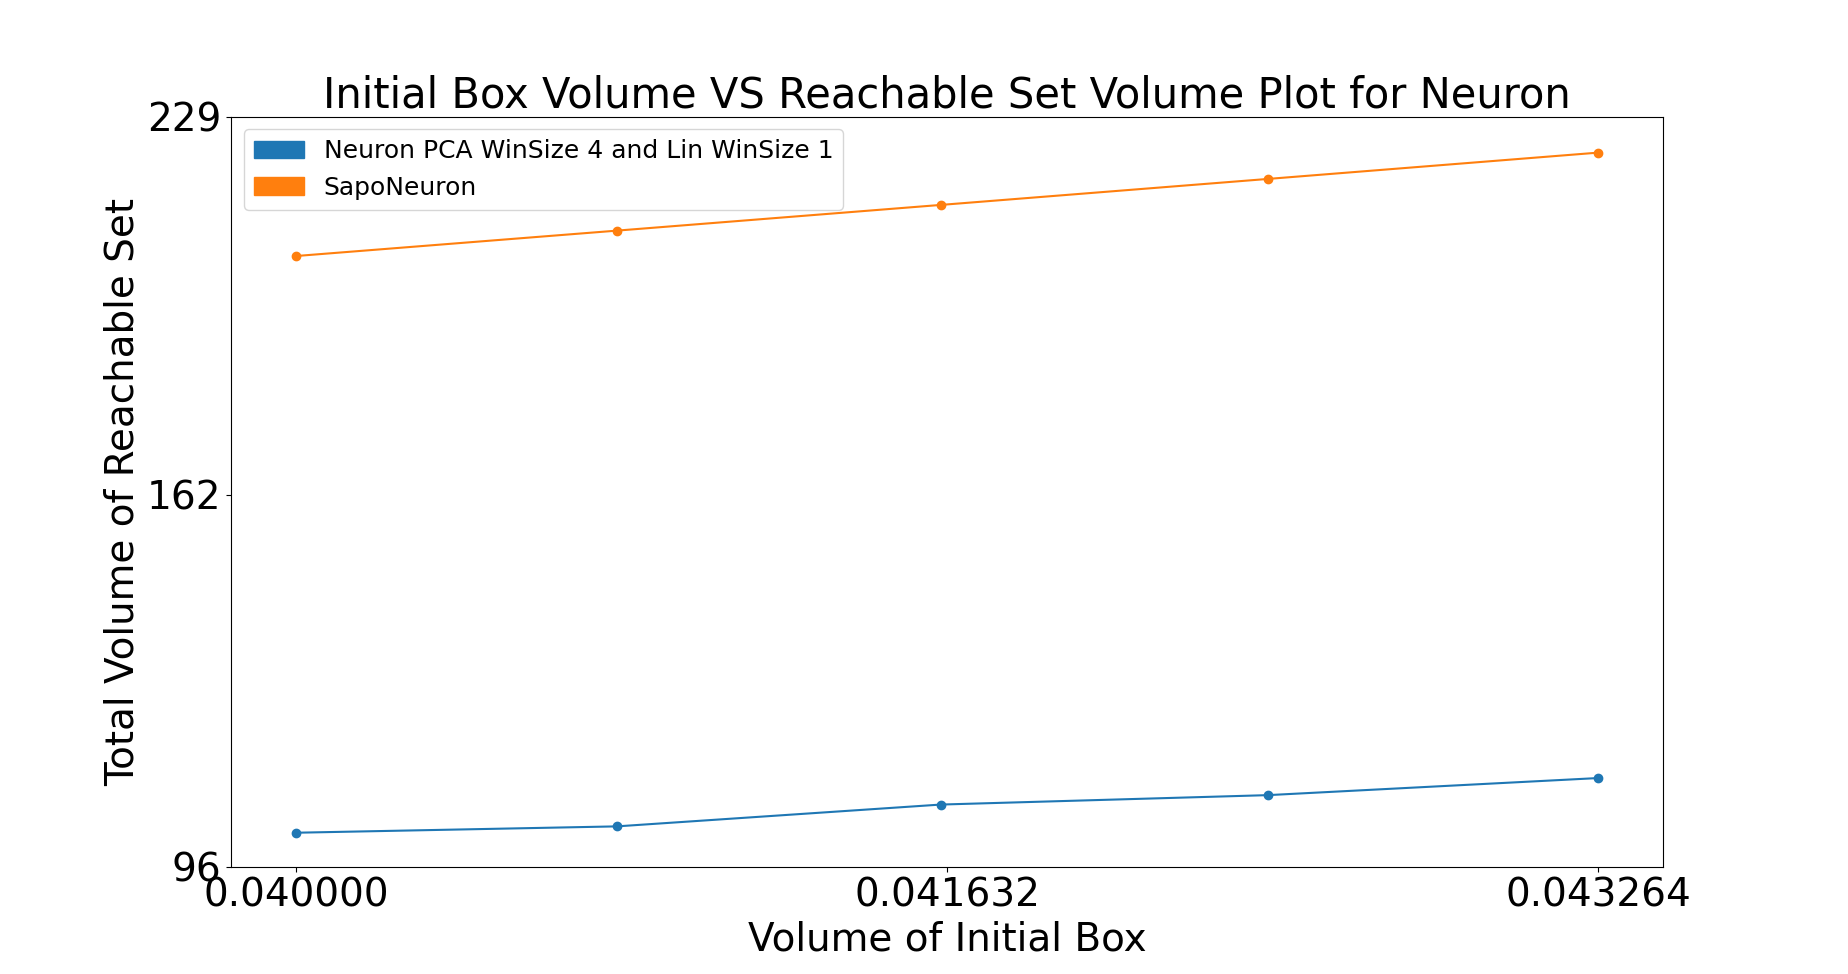
\includegraphics[width=\initvolwidth\textwidth, height=\initvolheight \textwidth]{figures/InitVolVSReachVol/NeuronInitReachVol200steps.png}
  }
  \subfloat[Coupled Vanderpol]{
  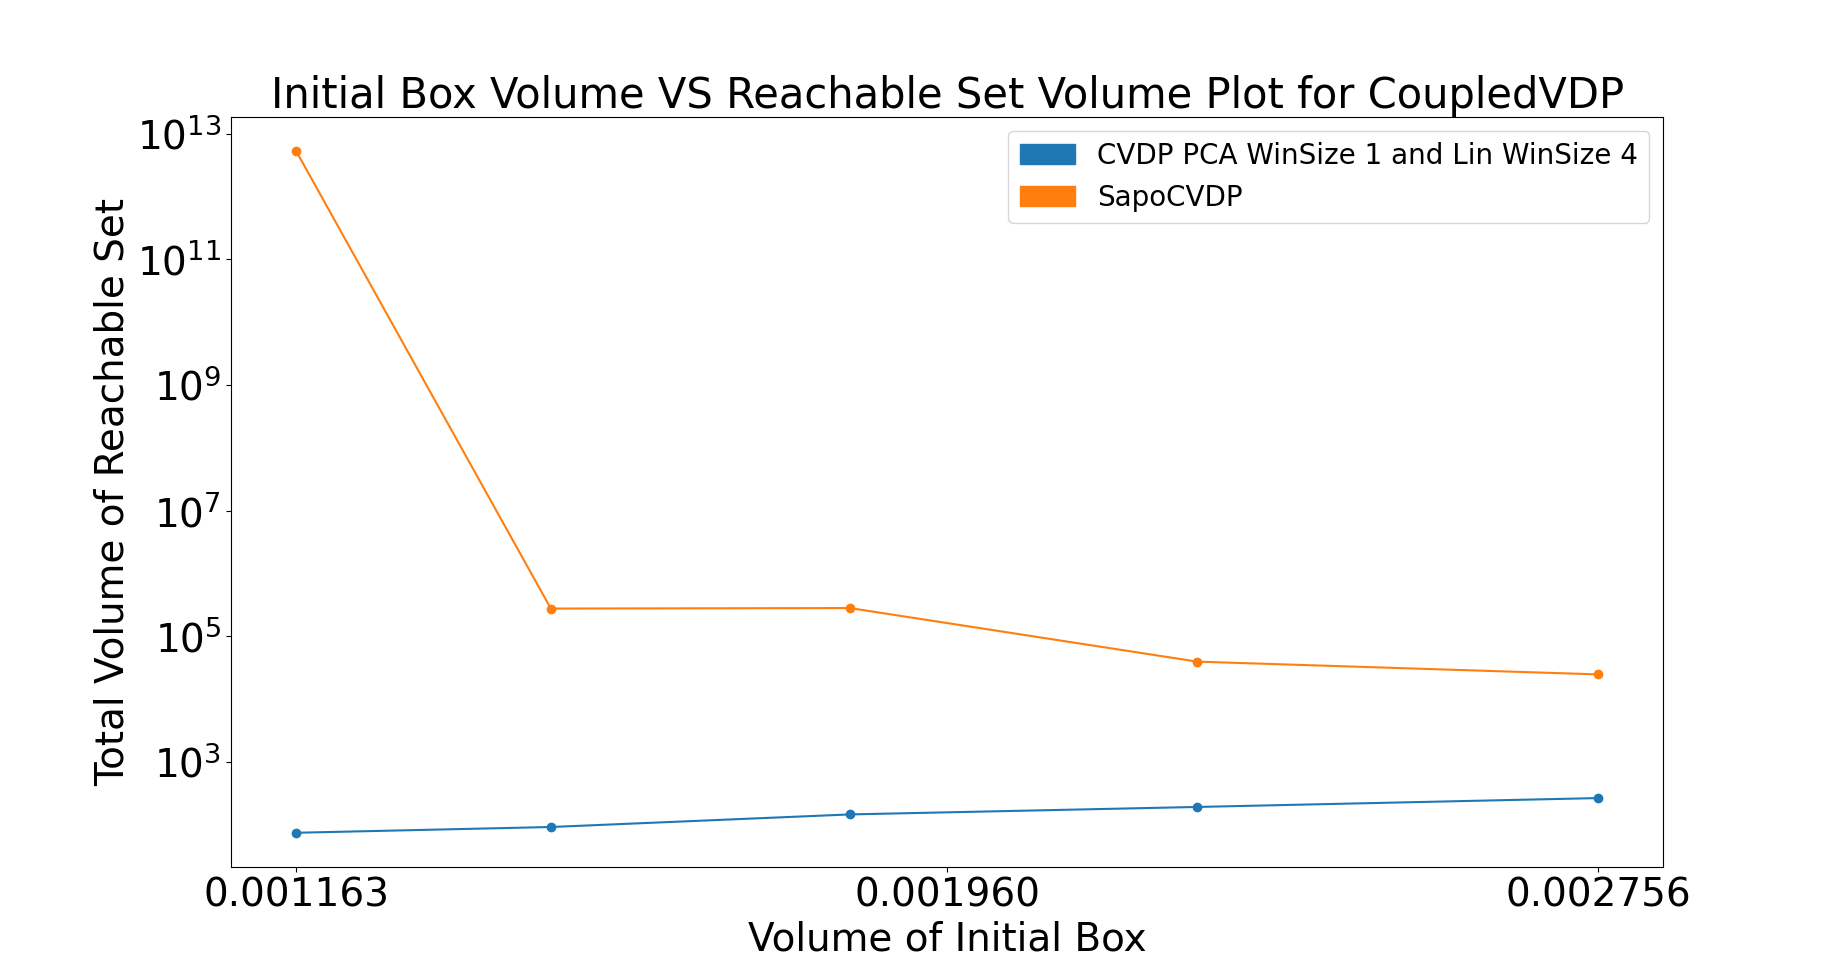
\includegraphics[width=\initvolwidth\textwidth, height=\initvolheight \textwidth]{figures/InitVolVSReachVol/CVDPInitReachVol.png}
  }

  \hspace*{\initvolhorshift}\subfloat[SIR]{
  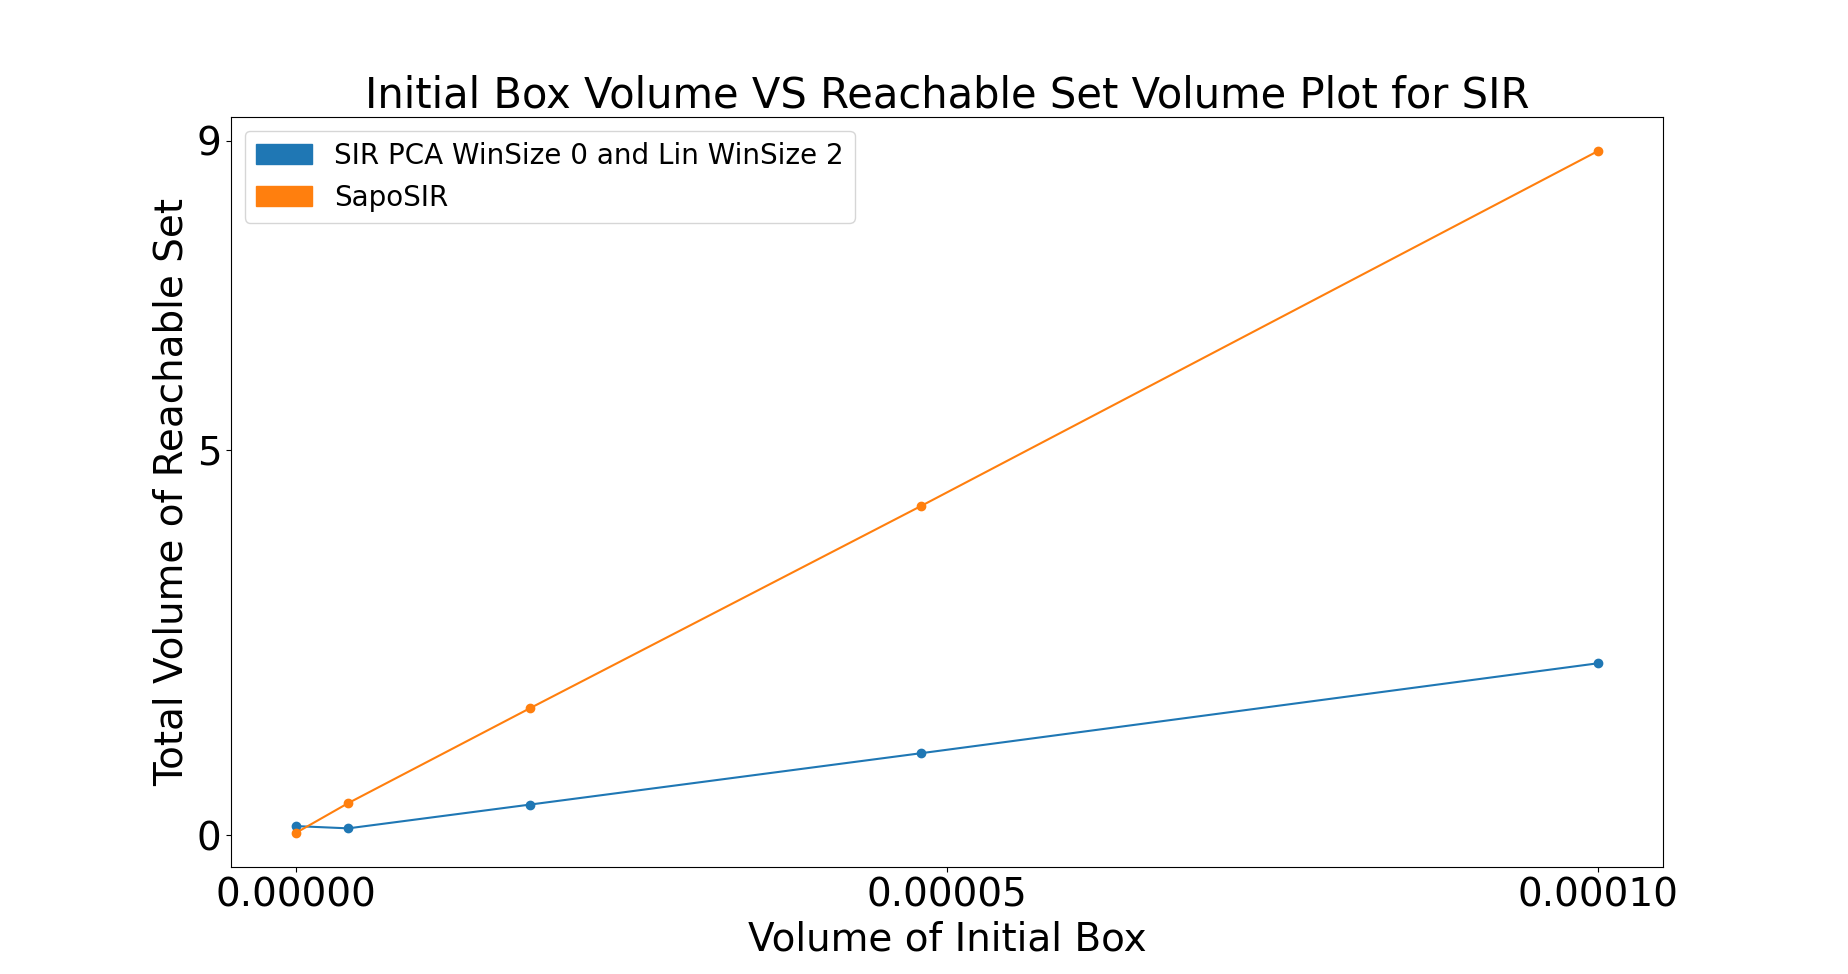
\includegraphics[width=\initvolwidth\textwidth, height=\initvolheight \textwidth]{figures/InitVolVSReachVol/SIRInitReachVol.png}
  }
  \subfloat[COVID]{
  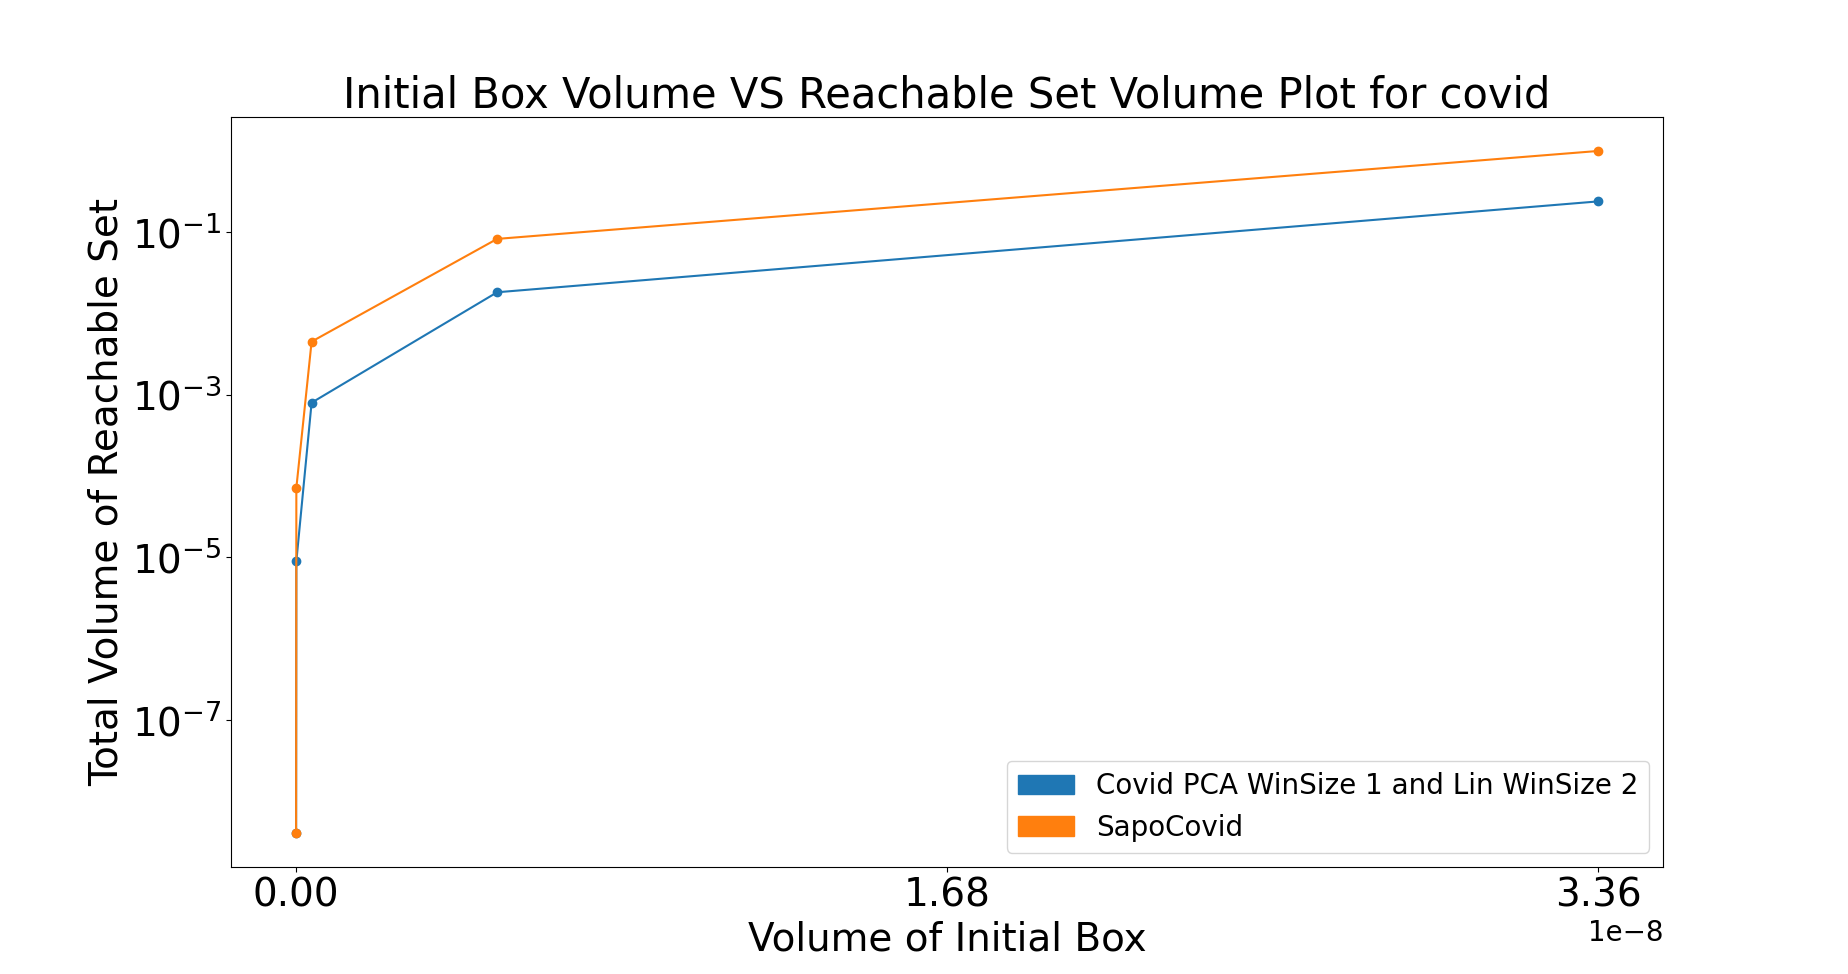
\includegraphics[width=\initvolwidth\textwidth, height=\initvolheight \textwidth]{figures/InitVolVSReachVol/CovidInitReachVol.png}
  }

  \caption{Comparison between the performance of diagonal static parallelotope bundles and that of the best performing dynamic parallelotope bundles as the volume of the initial set grows.}
  \label{fig:InitVolReachComp}
\end{figure}
